\scanpage{62}
correspondant, sur la sphère standard, à la région ci-contre, délimitée par le contour
\[
P_+Q_1R_0^-\unsure{S_0^+|D_0^+}R_0^+S_0^-P_-Q_\infty R_1^-S_1^+P_+
\]
\figure{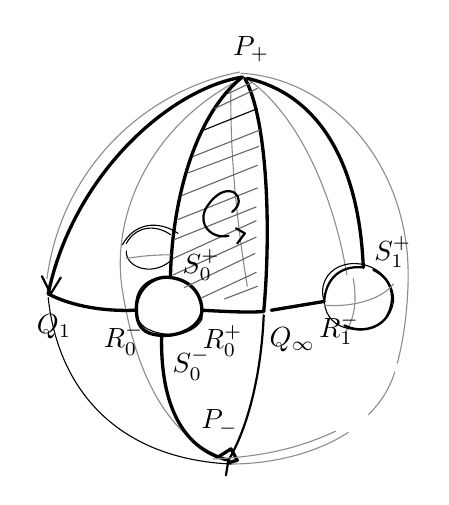
\begin{tikzpicture}[x=.016cm,y=-.016cm,line cap=round,line join=round]
\draw[thin,black!45] (219,104) .. controls (280,107) and (339,159) .. (350,239) .. controls (354,268) and (350,308) .. (343,334);
\draw[thin,black!45] (341,341) .. controls (337,354) and (330,365) .. (320,375);
\draw[thin,black!45] (304,389) .. controls (281,404) and (247,414) .. (211,414);
\draw[thin] (211,414) .. controls (123,410) and (74,357) .. (66,282);
\draw[thin,black!45] (65,267) .. controls (77,177) and (145,117) .. (218,103);
\draw[thin,black!45] (218,109) .. controls (146,146) and (115,218) .. (125,277) .. controls (136,346) and (163,395) .. (208,410);
\draw[thin,black!45] (225,109) .. controls (269,141) and (294,209) .. (303,264);
\draw[thin,black!45] (308,267) .. controls (312,288) and (307,302) .. (302,309);
\draw[thin,black!45] (211,112) .. controls (210,163) and (215,219) .. (224,273);
\draw[very thick] (220,107) .. controls (160,117) and (85,187) .. (66,279);
\draw[thick] (61,265) -- (68,279) -- (76,266);
\draw[very thick] (66,279) .. controls (85,289) and (111,293) .. (135,292);
\draw[very thick] (220,107) .. controls (180,139) and (164,211) .. (163,266);
\draw[very thick] (222,108) .. controls (240,140) and (243,228) .. (237,293);
\draw[very thick] (188,292) .. controls (207,293) and (225,294) .. (237,293);
\draw[very thick] (243,292) -- (285,285);
\draw[very thick] (224,108) .. controls (285,122) and (313,182) .. (316,258);
\draw[thin] (136,292) .. controls (133,274) and (147,264) .. (163,266) .. controls (180,269) and (190,282) .. (188,299) .. controls (182,311) and (162,315) .. (145,307) .. controls (138,303) and (135,297) .. (136,292);
\draw[very thick] (136,292) .. controls (135,277) and (148,264) .. (163,266) .. controls (179,268) and (188,279) .. (188,293);
\draw[very thick] (188,293) .. controls (186,307) and (166,315) .. (149,311) .. controls (140,309) and (136,302) .. (136,292);
\draw[thin] (128,239) .. controls (135,226) and (150,223) .. (163,232);
\draw[thin] (128,245) .. controls (127,257) and (147,266) .. (163,253);
\draw[thin] (125,240) .. controls (134,223) and (153,220) .. (169,231);
\draw[thin,black!45] (128,251) .. controls (139,249) and (151,248) .. (163,248);
\draw[thin] (285,285) .. controls (280,270) and (290,256) .. (307,255) .. controls (326,254) and (341,269) .. (340,285) .. controls (337,303) and (322,310) .. (307,307) .. controls (293,305) and (286,297) .. (285,285);
\draw[thick] (285,285) .. controls (286,268) and (297,256) .. (316,258);
\draw[thick] (324,260) .. controls (339,267) and (343,283) .. (334,298) .. controls (327,307) and (313,310) .. (301,304);
\draw[thin,black!45] (285,288) .. controls (310,290) and (332,282) .. (340,271);
\draw[very thick] (156,313) .. controls (155,364) and (171,402) .. (209,411);
\draw[thick] (237,296) .. controls (235,344) and (224,386) .. (209,411) -- (207,423);
\draw[very thick] (200,409) -- (211,402) -- (216,411) -- (209,413);
\draw[thin,black!45] (197,410) .. controls (242,408) and (270,399) .. (294,388);
\draw[thin,black!60] (209,120) -- (228,111);
\draw[thin,black!60] (198,132) -- (232,116);
\draw[thin] (187,150) -- (232,132);
\draw[thin,black!60] (181,170) -- (234,149);
\draw[thin,black!60] (177,183) -- (233,162);
\draw[thin,black!60] (172,201) -- (232,177);
\draw[thin,black!60] (169,220) -- (232,195);
\draw[thin,black!60] (166,236) -- (231,210);
\draw[thin,black!60] (165,251) -- (231,221);
\draw[thin,black!60] (165,264) -- (231,234);
\draw[thin,black!60] (174,274) -- (230,247);
\draw[thin,black!60] (188,282) -- (231,262);
\draw[thin,black!60] (206,283) -- (232,273);
\draw[thick] (212,214) .. controls (226,203) and (209,187) .. (194,207) .. controls (182,221) and (194,236) .. (209,233);
\draw[thick] (215,227) -- (222,231) -- (216,239);
\node[anchor=south] at (227,103) {$P_+$};
\node[anchor=east] at (92,305) {$Q_1$};
\node[anchor=north] at (126,295) {$R_0^-$};
\node[anchor=north west] at (181,296) {$R_0^+$};
\node[anchor=west] at (165,256) {$S_0^+$};
\node[anchor=north west] at (157,315) {$S_0^-$};
\node[anchor=north west] at (234,298) {$Q_\infty$};
\node[anchor=north] at (297,287) {$R_1^-$};
\node[anchor=west] at (317,246) {$S_1^+$};
\node[anchor=south] at (202,399) {$P_-$};
\end{tikzpicture}}
Les régions $\widetilde\Sigma_r$ sont permutées de façon simplement transitive par $\Gamma=G_J\times(1,\tau)$. Elles sont simplement connexes, et permettent donc de définir des
\[
\deleted{(42)}\qquad\Pi_r=\Pi_i^{\omega\varepsilon}=\Pi_1(\widetilde\Sigma;\widetilde\Sigma_r)=\Pi_1(\Sigma^*;\Sigma_r^*)
\]
\deleted{et des iso} \deleted{\unsure{qui}} mais qui sont reliés par un syst. transitif d'iso. à l'aide du gr. de $\Gamma$, de sorte qu'on peut identifier tous ces groupes entre eux. En fait, on trouve des isom. d'épinglage
\[
(42)\qquad\Psi_r:\Pi_{0,3}\longrightarrow\Pi_r=\Pi_i^{\omega,i}=\Pi_1(\widetilde\Sigma;\widetilde\Sigma_r)
\]
($\psi_r$ majuscule

\deleted{en \unsure{identi|ident}}
en composant
\diagram{\begin{tikzcd}[ampersand replacement=\&,column sep=large]
\Pi_{03}\arrow[r,shorten >=1.7em]\arrow[r,"\psi_r=\psi_\varepsilon^{\omega,i}"]\&
\begin{array}{c}
\Pi_1(\deleted{\unsure{P_\varepsilon|\Pi_\varepsilon}}\widetilde\Sigma,P_\varepsilon)\\
\simeq\Pi_1(\Sigma^*,P_\varepsilon)
\end{array}
\arrow[r,leftrightarrow,"\varphi_r^{-1}"]\&\Pi_r
\end{tikzcd}}
où $\deleted{\unsure{\varphi_r|\varphi}}$
\[
\varphi_r:\Pi_r\longrightarrow\Pi_\varepsilon=\Pi_1(\widetilde\Sigma,P_\varepsilon)
\]
est ``l\unsure{\deleted{a}|a}\unsure{''}'isomorphisme de transition'' correspondant à la région $1$-connexe $\Sigma_r$, et au point $P_\varepsilon$ de $\Sigma_r$.
\margin{61}
